\documentclass[12pt, twoside]{article}
\usepackage[francais]{babel}
\usepackage[T1]{fontenc}
\usepackage[latin1]{inputenc}
\usepackage[left=7mm, right=7mm, top=5mm, bottom=5mm]{geometry}
\usepackage{float}
\usepackage{graphicx}
\usepackage{array}
\usepackage{multirow}
\usepackage{amsmath,amssymb,mathrsfs}
\usepackage{soul}
\usepackage{textcomp}
\usepackage{eurosym}
 \usepackage{variations}
\usepackage{tabvar}


\pagestyle{empty}

\begin{document}


\section*{\center{Devoir maison 4}}

\medskip




\begin{center}
\fbox{

\textit{Devoir � rendre sur feuille grand format pour 
\textbf{vendredi 7 f�vrier 2014}.}

}
\end{center}

\enskip

\ul{Exercice 1}: \textit{(4,5 points)}

\enskip

\begin{tabular}{cc}
\begin{minipage}{13cm}
Les droites (TP) et (YG) sont s�cantes en I. On donne les longueurs:

IP= 5 cm; IG=7 cm ; IY=1,4 cm; YT=0,8 cm et TI=1 cm.

\begin{enumerate}
  \item Montrer que les droites (PG) et (YT) sont parall�les.
  \item Calculer le p�rim�tre du triangle IGP.
\end{enumerate}
\end{minipage}
&
\begin{minipage}{6cm}
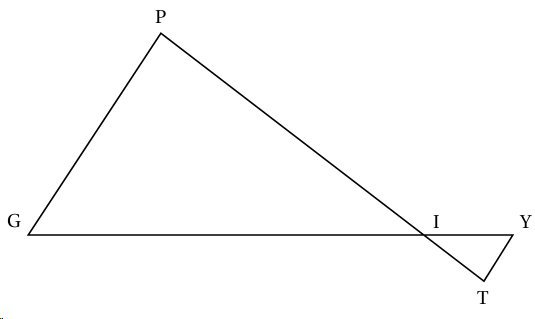
\includegraphics[width=5cm]{images/ex1.jpg}
\end{minipage}
\end{tabular}


\bigskip


\ul{Exercice 2}: \textit{(10 points dont 2 pour la construction)}

\enskip

\begin{enumerate}
  \item Construire un triangle ABC v�rifiant AB=7,5 cm; BC=10 cm et AC=12,5 cm.
  \item 
\begin{enumerate}
  \item Construire le point F appartenant au segment [AC] tel que CF=5
cm. 
\item  Construire le point G appartenant au segment [BC] tel que CG=4cm.
\end{enumerate}
  \item Prouver que le triangle ABC est rectangle en B.
  \item Les droites (AB) et (FG) sont-elles parall�les? Justifier votre r�ponse.
  \item Calculer FG.
  \item Que peut-on dire des droites (FG) et (BC)? Justifier votre r�ponse. 
\end{enumerate}


\bigskip


\ul{Exercice 3}: \textit{(3,5 points)}

\enskip

R�soudre les �quations suivantes:


\enskip

$22t+5=-10t-9$ 

\enskip

 $25-(2b-7)+4b=14+(6b-2)$ 

\enskip

$-8(5y+3)-4=6(2y-7)+5$


\bigskip

\ul{Exercice 4}: \textit{(3 points)}

\enskip


Sarah, David et Juliette sont fr�res et soeurs. Sarah a trois ans de plus que
Juliette. David est deux fois plus �g� que Sarah. En additionnant l'�ge de ces
trois enfants, on obtient sept fois l'�ge de Juliette. Quel est l'�ge de
Juliette?
\end{document}
